\documentclass[../main]{subfiles}
\begin{document}

\section{ESCALAS}
\begin{figure}[ht]
    \centering
    
\includegraphics[width=0.9\textwidth]{images/02/dibujo-escalas.png}
    \caption{Escalas en Dibujo Técnico.}
    \label{fig:escalas}
\end{figure}

\subsubsection*{Definición.}

La Escala (o escalas) en dibujo técnico y otros tipos de representaciones gráficas se define como la relación existente entre las dimensiones de la representación del objeto en el plano y las dimensiones reales del mismo, en una representación cartográfica, gráfica, fotográfica o modelo reducido.

\subsubsection*{Concepto de escala}

\begin{figure}[ht]
    \centering
    
\includegraphics[width=0.7\textwidth]{images/02/clip_image002.jpg}
    \caption{Escalas en dibujo}
    \label{fig:escalas2}
\end{figure}
La escala es uno de los instrumentos más importantes para la confección de dibujos. A veces podemos denominar como escala a cualquier regla graduada.

Según el uso que tienen las escalas en el dibujo técnico se define como \emph{la relación existente entre las dimensiones de la representación del artículo en el plano y las dimensiones reales del mismo.}

\begin{equation}
    Escala = \frac {\textit{Medida en Dibujo}}{ \textit{Medida Objeto Real}} = \textit{Medida en Dibujo}:\textit{Medida Objeto Real}
\end{equation}

\begin{equation}
    \textit{Medida en Dibujo}= \textit{Medida Objeto Real}\times Escala
\end{equation}

\begin{equation}
    \textit{Medida Objeto Real} = \frac {\textit{Medida en Dibujo}}{Escala} =
\end{equation}


\underline{Clasificación}
Según la aplicación en el dibujo, se establecen tres tipos:
\begin{itemize}
\item Escala de ampliación: las medidas del dibujo son mayores a las del objeto real.
\item Escala natural: las medidas del objeto y su representación en el plano son iguales.
\item Escala de reducción: las medidas del dibujo son menores las medidas del objeto real.
\end{itemize}


\underline{Distintas formas de expresión de las escalas}

Las escalas desde el punto de vista matemático, se expresan de diversas formas:
\begin{itemize}
\item Como fracción representativa:
1/2, 1/100, 1/5000, etc o 1:2, 1:100, ó 1:5000

\item Como igualdades o equivalencias:
4cm= 200m, 1cm= 10m

\item En forma gráfica, por ejemplo de barras o transversales.
\end{itemize}


\subsubsection*{Escalas gráficas}

\underline{La escala en los diversos campos del Dibujo Técnico}

En todo proyecto técnico está presente el uso de las escalas, así podemos mencionar el dibujo mecánico, el dibujo arquitectónico y el topográfico entre otros. En dependencia de las dimensiones del objeto a representar en el plano así será la escala a utilizar

El uso de las escalas además, responde a la actividad de normalización que establecen las Normas ISO para el intercambio internacional.

\subsubsection*{Determinación de escala}
\begin{figure}[ht]
    \centering
    
\includegraphics[width=0.9\textwidth]{images/02/1a.png}
\end{figure}
\newpage

\subsubsection*{Actividades:}
\begin{enumerate}
    \item ¿Qué entiende por escala y cómo se clasifican?
   
   
    \item Resolver los siguientes problemas:
    \begin{enumerate}
    \item En un plano de carreteras realizado a escala 1:50000,
la distancia entre dos ciudades, medida con una regla
graduada es de 45 mm. ¿Cuál será la distancia real
expresada en kilómetros?
    \item Un alumno va a realizar un plano de su habitación a escala 1:20, si su habitación tiene 5m de largo. ¿Cuánto deberá medir en el plano?
    \item El ancho real de una autopista es de 24 metros. Si el
plano en el que se encuentra dibujada está a escala 1:200,
¿cuántos milímetros tendrá de ancho en el dibujo?
   \item  A qué escala estará dibujado el plano de la escuela, si
sabemos que la puerta principal de entrada tiene de ancho
3,40 m, y en el plano hemos medido con la regla 68 mm. 
 \item - Si mide un barco mide 21 metros y su dibujo mide 70cm ¿A qué escala se realizó el dibujo?
    \end{enumerate}
  \item Dibujar las siguientes imágenes en escala 1:2, 1:1 y 2:1, en la siguiente página.
   \begin{figure}[ht]
        \centering
        
\includegraphics[width=0.5\textwidth]{images/02/dibujo-escalas-01.png}
    \end{figure}
\end{enumerate}
\newpage
\begin{tikzpicture}[remember picture, overlay, shift={(-3.6,-27.7)}]
\draw [step=0.5,gray, thin] (2.5,4.5) grid (20,28.5) ;
\end{tikzpicture}

\end{document}